\documentclass[10.5pt]{ctexart}
\usepackage{graphicx}
\usepackage[a4paper, inner=1.5cm, outer=3cm, top=2cm, bottom=3cm, bindingoffset=1cm]{geometry}
\usepackage{subcaption}
\begin{document}
\title{\textbf{\fontsize{15.75pt}{\baselineskip}{在Microsoft Word设置给俄语元音字母添加重音快捷键的操作步骤}}} 
\author{\fontsize{12pt}{\baselineskip}{数33 赵丰}}
\maketitle
本文使用的Microsoft Word版本是2016英文版,其他版本可类比该版本进行设置。
\begin{enumerate}
\item 启用宏(Macro)
\begin{figure}[!ht]
\centering
\begin{subfigure}[b]{0.4\textwidth}
        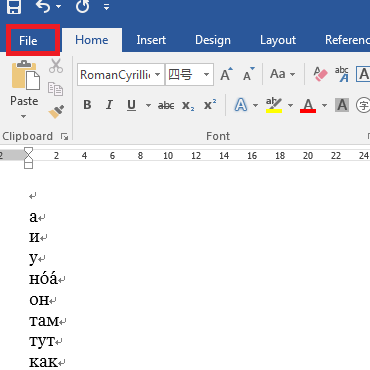
\includegraphics[width=\textwidth]{figure1.png}
        \caption{打开文件}
        \label{openFile}
\end{subfigure}\qquad	
\begin{subfigure}[b]{0.4\textwidth}
        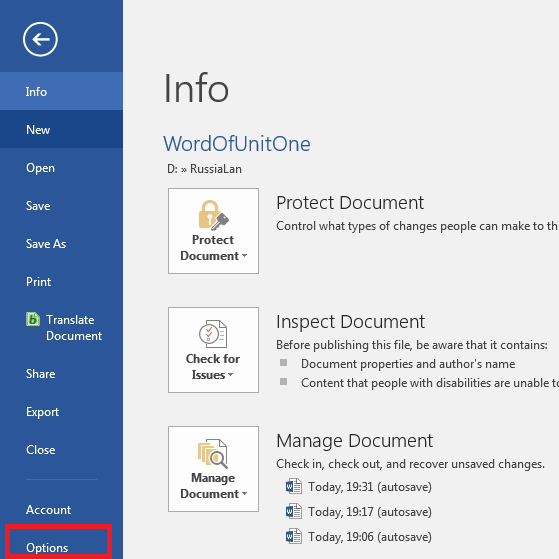
\includegraphics[width=\textwidth]{figure2.png}
        \caption{打开选项}
        \label{openOption}
\end{subfigure}
\begin{subfigure}[b]{0.4\textwidth}
        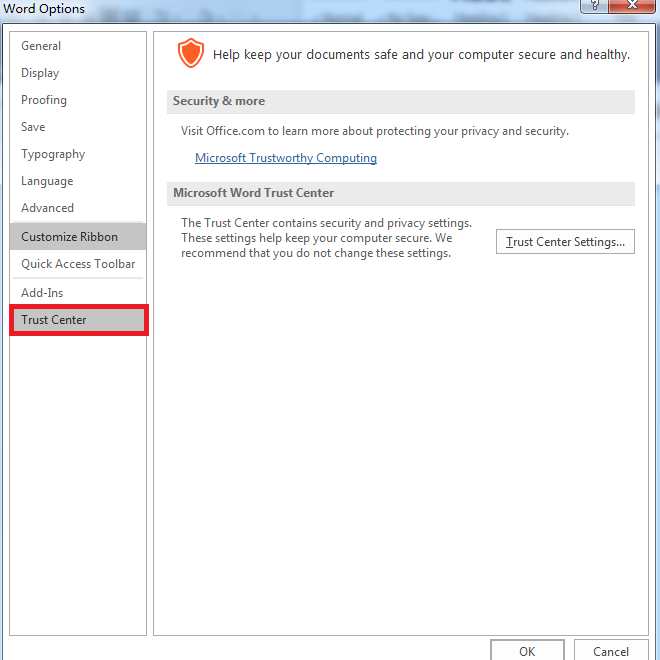
\includegraphics[width=\textwidth]{figure3.png}
        \caption{打开信任中心}
\end{subfigure}\qquad	
\begin{subfigure}[b]{0.4\textwidth}
        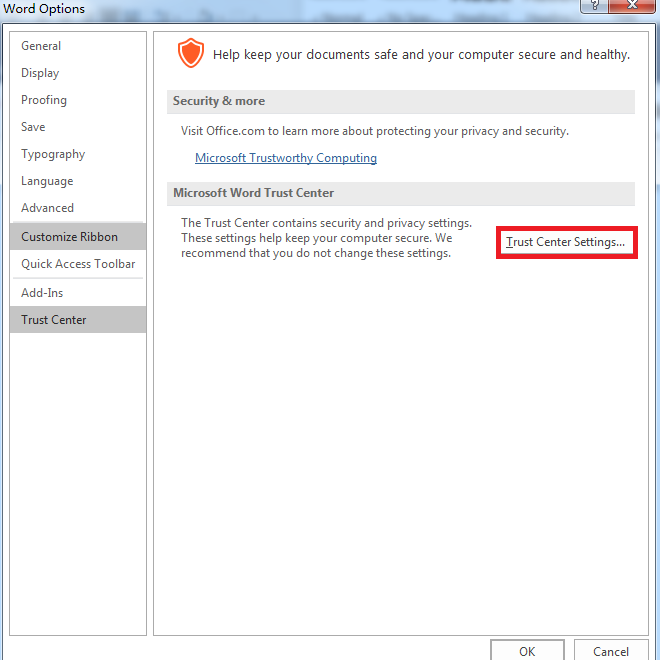
\includegraphics[width=\textwidth]{figure4.png}
        \caption{打开信任中心选项}
\end{subfigure}\\
图一
\end{figure}
\newpage
\item 启用开发工具(Developer)
\begin{figure}[!ht]
\centering
\begin{subfigure}[b]{0.4\textwidth}
        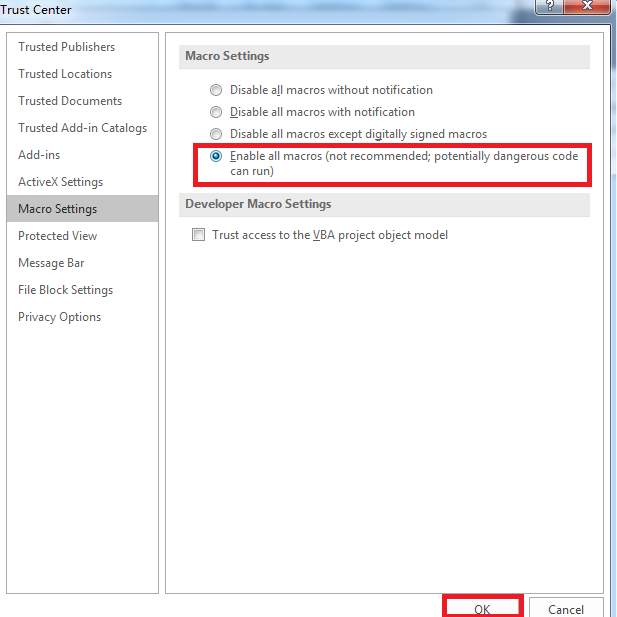
\includegraphics[width=\textwidth]{figure5.png}
        \caption{启用所有的宏并确定}
\end{subfigure}\qquad	
\begin{subfigure}[b]{0.4\textwidth}
        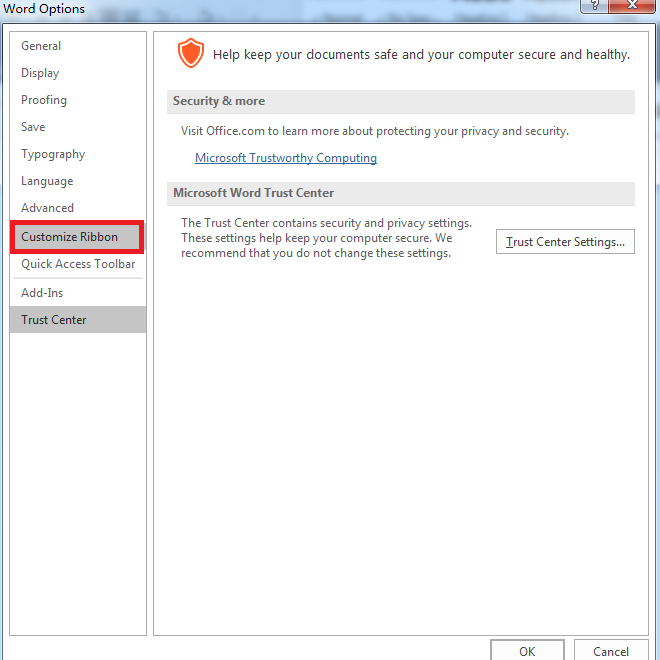
\includegraphics[width=\textwidth]{figure6.png}
        \caption{打开自定义功能区}
\end{subfigure}
\begin{subfigure}[b]{0.4\textwidth}
        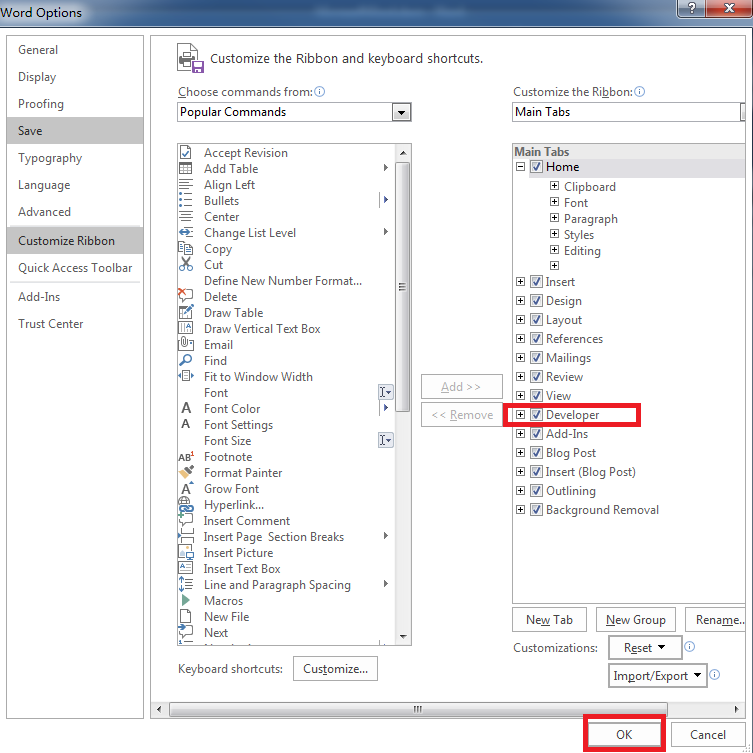
\includegraphics[width=\textwidth]{figure7.png}
        \caption{在开发者选项选框内打勾并确定}
\end{subfigure}\qquad	
\begin{subfigure}[b]{0.4\textwidth}
        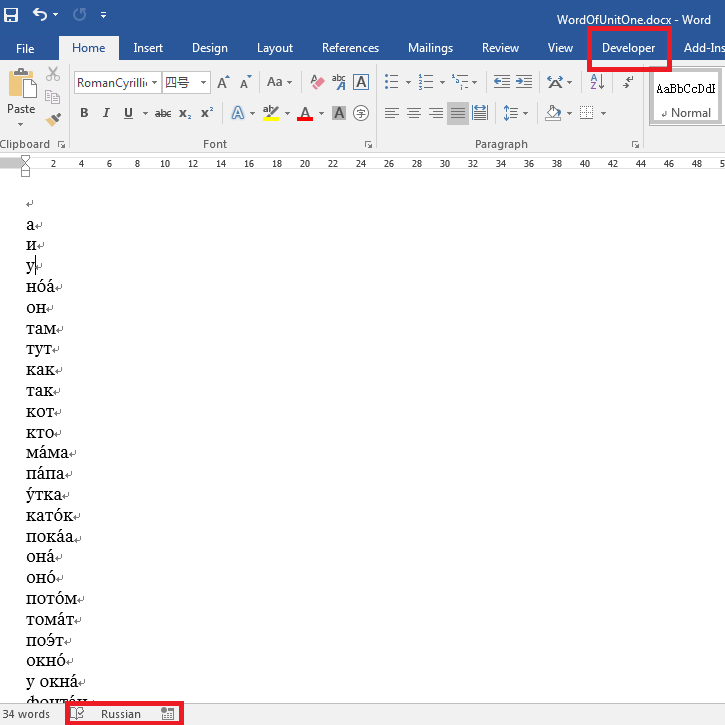
\includegraphics[width=\textwidth]{figure8.png}
        \caption{找到开发者卷展栏并进入}
\end{subfigure}\\
图二
\end{figure}
\newpage
\item 录制宏(Record Macro)
\begin{figure}[!ht]
\centering
\begin{subfigure}[b]{0.4\textwidth}
        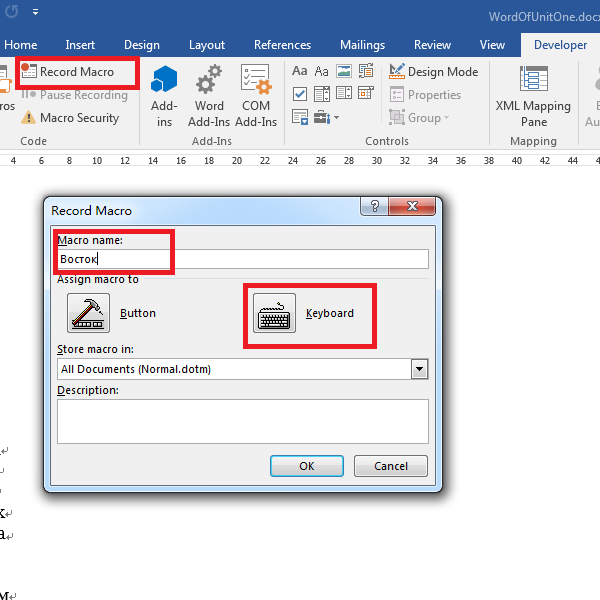
\includegraphics[width=\textwidth]{figure9.png}
        \caption{点击录制宏按扭,输入宏的名称并打开键盘快捷键设置}
\end{subfigure}\qquad	
\begin{subfigure}[b]{0.4\textwidth}
        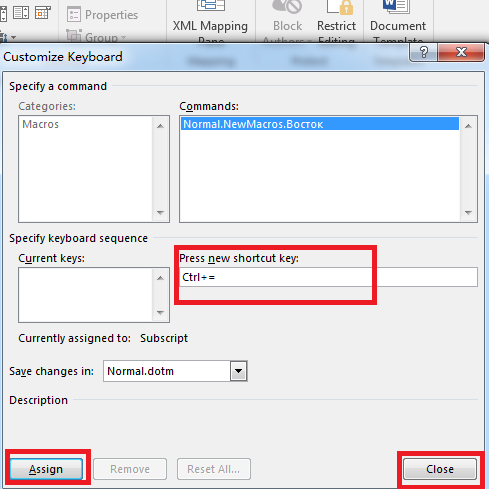
\includegraphics[width=\textwidth]{figure10.png}
        \caption{在输入新的快捷键的文本框中长按Ctrl再按加号并应用设置然后关闭对话框}
\end{subfigure}
\begin{subfigure}[b]{0.4\textwidth}
        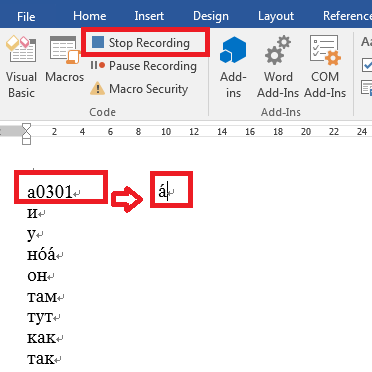
\includegraphics[width=\textwidth]{figure11.png}
        \caption{在某个元音字母后输入0301并长按Alt再按字母X,再按停止录制按扭}
\end{subfigure}\qquad	
\begin{subfigure}[b]{0.4\textwidth}
        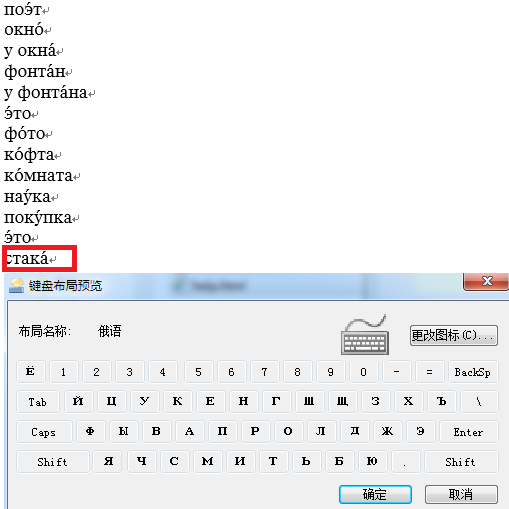
\includegraphics[width=\textwidth]{figure12.png}
        \caption{下次输入时在元音字母后长按Ctrl再按加号即可输入重音符号}
\end{subfigure}\\
图三
\end{figure}
\end{enumerate}

\end{document}